\chapter{Stärke in Zahlen}
\label{les:15}

\begin{chapquote}{Lewis Carroll, \textit{Alice im Wunderland}}
\enquote{Mal sehen: Viermal fünf ist zwölf, und viermal sechs ist dreizehn, und
viermal sieben ist vierzehn – oh je! Auf diese Weise komme ich ja nie bis
Zwanzig!}
\end{chapquote}

Zahlen sind ein wesentlicher Bestandteil unseres alltäglichen Lebens. Die
meisten von uns sind jedoch nicht recht gut mit großen Zahlen vertraut. Die
größten Zahlen denen wir im täglichen Leben begegnen, liegen in der
Größenordnung von Millionen, Milliarden oder Billionen. Wir können über
Millionen von Menschen in Armut oder Milliarden von Dollar die für die
Rettungsschirme für Banken ausgegeben werden oder gar über Trillionen von
Staatsschulden lesen. Auch wenn es schwer ist diese Schlagzeilen zu
interpretieren, können wir Zahlen dieser Größenordnung gewissermaßen einordnen.

Obwohl wir mit Milliarden und Billionen noch etwas anfangen können, beginnt
unsere Intuition bereits bei Zahlen der Größenordnung Milliarden zu versagen.
Hast du eine Ahnung, wie lange du warten müsstest bis eine Million / Milliarde
/ Billion Sekunden vergehen? Wenn du nur ein bisschen wie ich bist, wärst du
jetzt verloren ohne das Ergebnis zu berechnen.

Betrachten wir folgendes Beispiel: Der Unterschied ist eine Erhöhung um drei
Zehnerpotenzen: $10^6$, $10^9$, $10^{12}$. In Sekunden zu denken bringt uns
nicht weiter also lass uns das in etwas übersetzen das wir verstehen:

\begin{itemize}
  \item $10^6$: Eine Million Sekunden war vor $1 \frac{1}{2}$ Wochen.
  \item $10^9$: Eine Milliarde Sekunden war vor fast 32 Jahren.
  \item $10^{12}$: Vor einer Billion Sekunden war Manhattan noch von einer
  dicken Eisschicht bedeckt.\footnote{Eine Billion Sekunden ($10^{12}$)
  entspricht $31.710$ Jahren. Das letzte Glazial setzte vor etwa 115.000 Jahren
  ein und endete vor etwa 11.700 Jahren.~\cite{wiki:LGM}}
\end{itemize}

\begin{figure}
  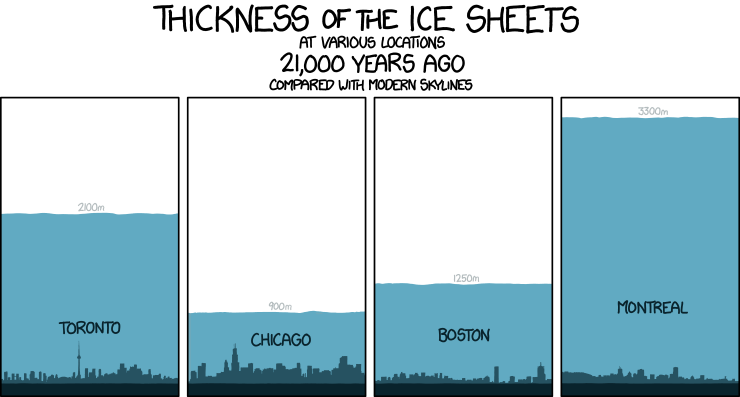
\includegraphics[width=\textwidth]{assets/images/xkcd-1225.png}
  \caption{Dicke der Eisschichten vor ungefähr einer Billion Sekunden. Quelle: xkcd 1225}
  \label{fig:xkcd-1225}
\end{figure}

Sobald wir in den Bereich der modernen Kryptographie eintreten, versagt unsere
Intuition katastrophal. Bitcoin wurde um große Zahlen herum aufgebaut: Als Basis dient
die Tatsache, dass es praktisch unmöglich ist, diese großen Zahlen zu erraten. Die Zahlen sind
weitaus größer als alles was uns im Alltag begegnen könnte. Viele Zehnerpotenzen
größer. Zu verstehen wie groß diese Zahlen wirklich sind, ist entscheidend für
das Verständnis von Bitcoin als großem Ganzen.

Nehmen wir SHA-256\footnote{SHA-256 ist Teil von SHA-2, eine Gruppe von
verschiedenen kryptologischen Hashfunktionen welche von der NSA entwickelt
wurde.~\cite{wiki:sha2}}, eine der in Bitcoin verwendeten
Hashfunktionen\footnote{Bitcoin verwendet SHA-256 als
Block-Hashing-Algorithmus.~\cite{btcwiki:block-hashing}} als konkretes Beispiel.
Es liegt in der Natur der Sache, bei 256 Bits an
\enquote{Zweihundertsechsundfünzig} zu denken, was an sich ja keine große Zahl
ist. Die Zahl in SHA-256 spricht jedoch von Potenzen -- etwas womit unser Gehirn
eben nicht sonderlich gut umgehen kann.

Während die Länge der Bits eine bequeme Metrik ist, geht die wahre Bedeutung der
256-Bit-Sicherheit durch diese Schreibweise verloren. Ähnlich wie bei den oben
genannten Millionen ($10^6$) und Milliarden ($10^9$) spricht die Zahl in SHA-256
von Größenordnungen ($2^{256}$).

Also, wie stark ist SHA-256 genau?

\begin{quotation}\begin{samepage}
\enquote{SHA-256 ist sehr stark. Es ist nicht wie der nächste Schritt von MD5 zu
SHA1. Es kann mehrere Jahrzehnte andauern, es sei denn es gibt einen massiven
technologischen Durchbruch.}
\begin{flushright} -- Satoshi Nakamoto\footnote{Satoshi Nakamoto, in einer
Antwort zu Fragen über SHA-256 Kollisionen. \cite{satoshi-sha256}}
\end{flushright}\end{samepage}\end{quotation}

Ausgeschrieben ergibt $2^{256}$ folgende Zahl:

\begin{quotation}\begin{samepage}
    115 Duodezilliarden 792 Duodezillionen 89 Undezilliarden 237 Undezillionen
    316 Dezilliarden 195 Dezillionen 423 Nonilliarden 570 Nonillionen 985
    Oktilliarden 8 Oktillionen 687 Septilliarden 907 Septillionen 853
    Sextilliarden 269 Sextillionen 984 Quintilliarden 665 Quintillionen 640
    Quadrilliarden 564 Quadrillionen 39 Trilliarden 457 Trillionen 584
    Billiarden 7 Billionen 913 Milliarden 129 Millionen 639 Tausend 936.
\end{samepage}\end{quotation}

Das sind viele Nonilliarden! Es ist schier unmöglich diese Zahl zu verstehen. Es
gibt nichts im physikalischen Universum womit man sie vergleichen könnte. Sie
ist weitaus größer als die Anzahl aller Atome im beobachtbaren Universum. Eine
Zahl von dieser Größenordnung ergibt einfach keinen Sinn für unser menschliches
Gehirn.

Eine der besten Visualisierungen der wahren Stärke von SHA-256 ist ein  Video
von Grant Sanderson. Mit dem treffenden Namen \textit{\enquote{Wie sicher ist
256-Bit-Sicherheit?}}\footnote{\url{https://youtu.be/S9JGmA5_unY}} Tu dir selbst
den Gefallen und nimm dir die fünf Minuten Zeit um es dir anzusehen. Wie alle
anderen 3Blue1Brown Videos ist es nicht nur faszinierend, sondern auch
außergewöhnlich gut gemacht. Warnung: Du könntest in einen Mathe-Kaninchenbau
fallen.

\begin{figure}
  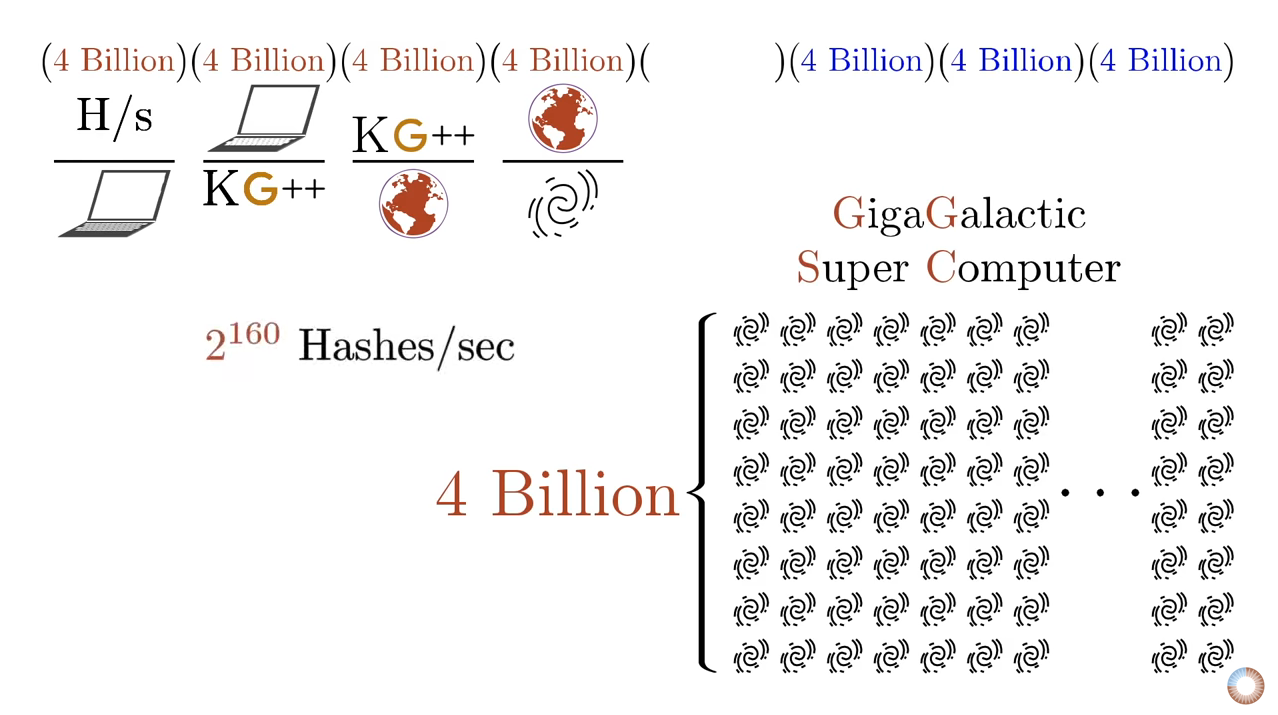
\includegraphics[width=\textwidth]{assets/images/youtube-vid-inverted.png}
  \caption{Illustration von den Sicherheitsgarantien von SHA-256. Grafik aus dem Video von Grant Sanderson / 3Blue1Brown.}
  \label{fig:youtube-vid-inverted}
\end{figure}

Bruce Schneier~\cite{web:schneier} nutzte die physikalischen Grenzen der
Rechenleistung von heutigen Computern um diese Zahl zu beschreiben: Selbst wenn
wir einen optimalen Computer bauen könnten, welcher jede verfügbare Energie
nutzen würde um Bits perfekt zu manipulieren~\cite{wiki:landauer}, eine
Dyson-Sphäre\footnote{Eine Dyson-Sphäre, benannt nach Freeman Dyson, ist ein
hypothetisches Konstrukt, welches die Energie eines Sterns absorbiert oder
umlenkt, um sie somit optimal nutzen zu können.~\cite{wiki:dyson}} um unsere
Sonne herum bauen und sie 100 Milliarden Milliarden Jahre lang laufen lassen
würden, hätten wir immer noch nur eine Chance von $25\%$ eine Nadel in einem
256-Bit-Heuhaufen zu finden.

\begin{quotation}\begin{samepage}
\enquote{Diese Zahlen haben nichts mit der Technologie der Geräte zu tun; sie
sind die Maxima, die die Thermodynamik zulässt. Und sie implizieren stark, dass
Brute-Force-Angriffe auf 256-Bit-Schlüssel nicht möglich sind, bis Computer aus
etwas anderem als Materie gebaut werden und etwas anderes als Raum belegen.}
\begin{flushright} -- Bruce Schneier\footnote{Bruce Schneier, \textit{Applied Cryptography} \cite{bruce-schneier}}
\end{flushright}\end{samepage}\end{quotation}

Es ist schwer die Tiefgängikeit dieser Aussage zu verdeutlichen. Starke
Kryptographie kehrt das Machtgleichgewicht der physischen Welt, an die wir so
gewöhnt sind, um. Dinge die man nicht knacken kann gibt es in der realen Welt
nicht. Wende genug Kraft auf und du kannst jede Tür, Box oder Schatzkiste
öffnen.

Die Schatzkiste von Bitcoin ist ganz anders. Sie wird durch eine starke
Kryptographie gesichert, die Brute-Force Angriffen nur wenige Chancen bietet.
Und solange die zugrunde liegenden mathematischen Annahmen Bestand haben, sind
Brute-Force Attacken alles was wir in unserem Arsenal haben. Zugegeben, es gibt
auch die Option eines globalen \$5-Schraubenschlüsselangriffs (siehe
Abbildung~\ref{fig:xkcd-538}). Aber Folter wird nicht bei allen Bitcoin-Adressen
funktionieren und die kryptographischen Wände Bitcoins werden weiterhin
Brute-Force-Angriffe abwehren. Selbst wenn du es mit der Kraft von tausend
Sonnen versuchst. Wortwörtlich.

\begin{figure}
  \centering
  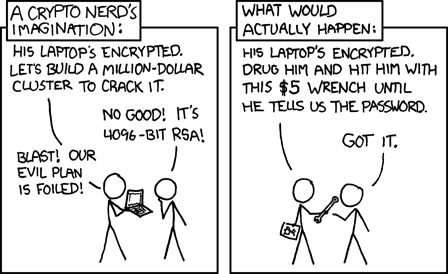
\includegraphics[width=8cm]{assets/images/xkcd-538.png}
  \caption{\$5-Schraubenschlüsselangriffs. Quelle: xkcd 538}
  \label{fig:xkcd-538}
\end{figure}

Diese Tatsache und ihre Auswirkungen wurden in dem \enquote{\textit{Call to
Cryptographic Arms}} (\enquote{Aufruf zu kryptographischen Waffen}) treffend
zusammengefasst: \textit{\enquote{Keine Menge an Zwang oder Gewalt wird jemals
ein mathematisches Problem lösen.}}

\begin{quotation}\begin{samepage}
\enquote{Es ist nicht offensichtlich, dass die Welt auf diese Weise
funktionieren musste. Aber irgendwie lächelt das Universum in Bezug auf
Verschlüsselung.}
\begin{flushright} -- Julian Assange\footnote{Julian Assange, \textit{A Call to Cryptographic Arms} \cite{call-to-cryptographic-arms}}
\end{flushright}\end{samepage}\end{quotation}

Noch weiß niemand genau, ob das Lächeln des Universums echt ist oder nicht. Es
ist möglich, dass unsere Annahmen von mathematischen Asymmetrien falsch sind und
wir feststellen, dass P tatsächlich gleich NP \cite{wiki:pnp} ist oder wir
finden überraschender Weise schnelle Lösungen für spezifische Probleme
\cite{wiki:discrete-log} von denen wir derzeit annehmen, dass sie sehr schwer
oder gar nicht lösbar sind. Sollte dies der Fall sein wird die Kryptographie,
wie wir sie kennen, aufhören zu existieren und die Auswirkungen würden
höchstwahrscheinlich die Welt bis zur Unkenntlichkeit verändern.

\begin{quotation}\begin{samepage}
\enquote{Vires in Numeris} = \enquote{Stärke in Zahlen}\footnote{\textit{Vires
in Numeris} wurde das erste Mal von BitcoinTalk-User \textit{epii} als
Bitcoin-Motto vorgeschlagen.~\cite{epii}}
\end{samepage}\end{quotation}

\textit{Vires in numeris} ist nicht nur ein einprägsames Motto der Bitcoiner.
Die Erkenntnis, dass es eine unergründliche Kraft gibt die in Zahlen zu finden
ist, ist tiefgründig. Das und die Umkehrung der bestehenden Machtverhältnisse zu
verstehen, veränderte meine Sicht auf die Welt und die Zukunft die vor uns
liegt.

Ein direktes Resultat dessen ist die Tatsache, dass man niemanden um Erlaubnis
bitten muss um an Bitcoin teilzunehmen. Es gibt keine Seite auf der man sich
anmelden muss, kein verantwortliches Unternehmen, keine Regierungsbehörde an die
man Antragsformulare senden muss. Erstelle dir einfach eine große Zahl und du
kannst direkt loslegen. Die zentrale Behörde für die Kontoerstellung ist die
Mathematik.

\begin{figure}
  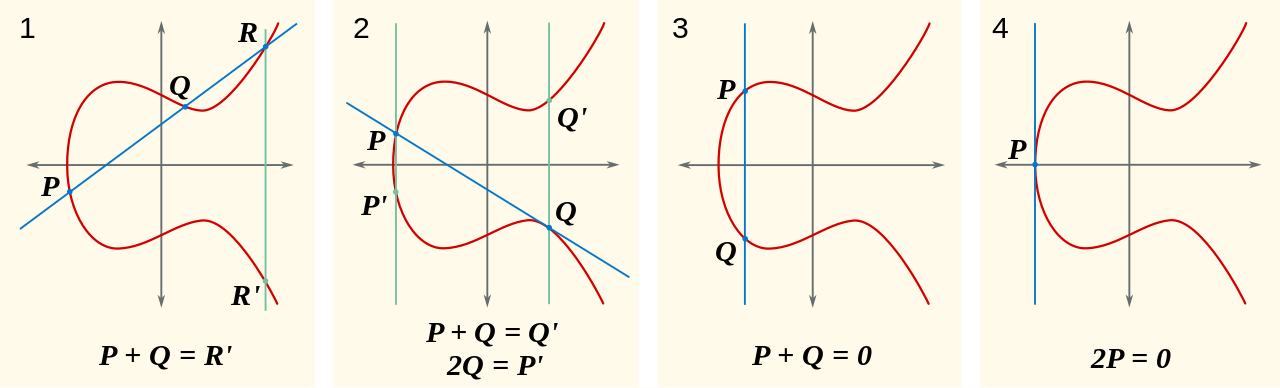
\includegraphics[width=\textwidth]{assets/images/elliptic-curve-examples.png}
  \caption{Grafische Darstellung elliptischer Kurven. Bild: cc-by-sa Emmanuel Boutet.}
  \label{fig:elliptic-curve-examples}
\end{figure}

Bitcoin basiert auf unserem besten Verständnis der Realität. Während es in der
Physik, Informatik und Mathematik noch viele offene Probleme gibt, sind wir uns
bei einigen Dingen ziemlich sicher. Dass es eine Asymmetrie zwischen dem Finden
von Lösungen und der Validierung der Richtigkeit dieser Lösungen gibt, ist eine
solche. Dass die Berechnung Energie benötigt ist eine andere. Mit anderen
Worten: Eine Nadel in einem Heuhaufen zu finden ist schwieriger, als zu prüfen
ob das spitze Ding in der Hand tatsächlich eine Nadel ist oder nicht. Und das
Finden der Nadel erfordert Arbeit.

Die Weite vom Raum der Bitcoinadressen ist wahrlich unbegreiflich. Die Anzahl
der möglichen privaten Schlüssel ist sogar noch größer. Es ist faszinierend wie
viel von unserer modernen Welt auf die Unwahrscheinlichkeit hinausläuft, eine
Nadel in einem unvorstellbar großen Heuhaufen zu finden. Ich bin mir dieser
Tatsache heute mehr denn je bewusst.

\paragraph{Bitcoin lehrte mich, dass eine unglaubliche Stärke in Zahlen steckt.}

% ---
%
% #### Down the Rabbit Hole
%
% - [How secure is 256 bit security?]["How secure is 256 bit security?"] by 3Blue1Brown
% - [Block Hashing Algorithm][hash functions] on the Bitcoin Wiki
% - [Last Glacial Maximum][thick layer of ice], [SHA-2][SHA-256], [Dyson Sphere][Dyson sphere], [Landauer's Principle][flip bits perfectly] [P versus NP][P actually equals NP], [Discrete Logarithm][specific problems] on Wikipedia
%
% [thick layer of ice]: https://en.wikipedia.org/wiki/Last_Glacial_Maximum
% [xkcd \#1125]: https://xkcd.com/1225/
% [SHA-256]: https://en.wikipedia.org/wiki/SHA-2
% [hash functions]: https://en.bitcoin.it/wiki/Block_hashing_algorithm
% ["How secure is 256 bit security?"]: https://www.youtube.com/watch?v=S9JGmA5_unY
% [Bruce Schneier]: https://www.schneier.com/
% [flip bits perfectly]: https://en.wikipedia.org/wiki/Landauer%27s_principle#Equation
% [Dyson sphere]: https://en.wikipedia.org/wiki/Dyson_sphere
% [2]: https://books.google.com/books?id=Ok0nDwAAQBAJ&pg=PT316&dq=%22These+numbers+have+nothing+to+do+with+the+technology+of+the+devices;%22&hl=en&sa=X&ved=0ahUKEwjXttWl8YLhAhUphOAKHZZOCcsQ6AEIKjAA#v=onepage&q&f=false
% [wrench attack]: https://xkcd.com/538/
% [call to cryptographic arms]: https://cryptome.org/2012/12/assange-crypto-arms.htm
% [P actually equals NP]: https://en.wikipedia.org/wiki/P_versus_NP_problem#P_=_NP
% [specific problems]: https://en.wikipedia.org/wiki/Discrete_logarithm#Cryptography
% [3Blue1Brown]: https://twitter.com/3blue1brown
%
% <!-- Wikipedia -->
% [alice]: https://en.wikipedia.org/wiki/Alice%27s_Adventures_in_Wonderland
% [carroll]: https://en.wikipedia.org/wiki/Lewis_Carroll
